% !TeX spellcheck = en_US
% !TeX encoding = utf8
% !TeX program = xelatex
% !BIB program = bibtex
% \documentclass[mathserif,compress,12pt]{ctexbeamer}
\documentclass[12pt,notes,mathserif]{beamer}
% \documentclass[draft]{beamer}	
\usetheme{Singapore}
% \usetheme{Hannover}
%\usepackage{pgfpages}
%\setbeameroption{show notes on second screen}

\usepackage[british]{babel}
\usepackage{graphicx,hyperref,url}
% \usepackage{ru}
\usepackage{mmstyles,bm,ulem,extpfeil}

\usepackage{listings}
\usefonttheme[onlymath]{serif}
\usepackage{fontspec}
\usepackage{xeCJK}
% \setCJKfamilyfont{hei}{SimHei}
% \setCJKmainfont[BoldFont=Arial, ItalicFont=Arial]{Arial}
% \pgfdeclareimage[width=\paperwidth,height=\paperheight]{bg}{background}
% \setbeamertemplate{background}{\pgfuseimage{bg}}
%% columns
\newcommand{\begincols}[1]{\begin{columns}{#1}}
\newcommand{\stopcols}{\end{columns}}
% \usepackage[backend=biber]{biblatex}
% \bibliography{./ref.bib}
%\addbibresource{ref.bib}
\usepackage{indentfirst}
\usepackage{longtable}
\usepackage{float}
%\usepackage{picins}
\usepackage{rotating}
\usepackage{subfigure}
\usepackage{tabu}
\usepackage{amsmath}
\usepackage{amssymb}
\usepackage{setspace}
\usepackage{amsfonts}
\usepackage{appendix}
\usepackage{listings}
\usepackage{xcolor}
\usepackage{colortbl}
\usepackage{geometry}
% \setCJKfamilyfont{cjkhwxk}{SimSun}
% \newcommand*{\cjkhwxk}{\CJKfamily{cjkhwxk}}
%\newfontfamily{\consolas}{Consolas}
%\newfontfamily{\monaco}{Monaco}
%\setmonofont[Mapping={}]{Consolas}	%英文引号之类的正常显示,相当于设置英文字体
%\setsansfont{Consolas} %设置英文字体 Monaco, Consolas,  Fantasque Sans Mono
% \setmainfont{Times New Roman}
% \newfontfamily{\consolas}{Times New Roman}
% \newfontfamily{\monaco}{Arial}
% \setCJKmainfont{Times New Roman}
%\setmainfont{MONACO.TTF}
%\setsansfont{MONACO.TTF}
\newcommand{\verylarge}{\fontsize{60pt}{\baselineskip}\selectfont}  
\newcommand{\chuhao}{\fontsize{44.9pt}{\baselineskip}\selectfont}  
\newcommand{\xiaochu}{\fontsize{38.5pt}{\baselineskip}\selectfont}  
\newcommand{\yihao}{\fontsize{27.8pt}{\baselineskip}\selectfont}  
\newcommand{\xiaoyi}{\fontsize{25.7pt}{\baselineskip}\selectfont}  
\newcommand{\erhao}{\fontsize{23.5pt}{\baselineskip}\selectfont}  
\newcommand{\xiaoerhao}{\fontsize{19.3pt}{\baselineskip}\selectfont} 
\newcommand{\sihao}{\fontsize{14pt}{\baselineskip}\selectfont}      % 字号设置  
\newcommand{\xiaosihao}{\fontsize{12pt}{\baselineskip}\selectfont}  % 字号设置  
\newcommand{\wuhao}{\fontsize{10.5pt}{\baselineskip}\selectfont}    % 字号设置  
\newcommand{\xiaowuhao}{\fontsize{9pt}{\baselineskip}\selectfont}   % 字号设置  
\newcommand{\liuhao}{\fontsize{7.875pt}{\baselineskip}\selectfont}  % 字号设置  
\newcommand{\qihao}{\fontsize{5.25pt}{\baselineskip}\selectfont}    % 字号设置 

\graphicspath{{./fig/}}

% \setbeamertemplate{footnote}{%
%   \hangpara{2em}{1}%
%   \makebox[2em][l]{\insertfootnotemark}\footnotesize\insertfootnotetext\par%
% }

\definecolor{cred}{rgb}{0.6,0,0}
\definecolor{cgreen}{rgb}{0.25,0.5,0.35}
\definecolor{cpurple}{rgb}{0.5,0,0.35}
\definecolor{cdocblue}{rgb}{0.25,0.35,0.75}
\definecolor{cdark}{rgb}{0.95,1.0,1.0}
\lstset{
	language=R,
	numbers=left,
	numberstyle=\tiny\color{black},
	keywordstyle=\color{cpurple}\consolas,
	commentstyle=\color{cgreen}\consolas,
	stringstyle=\color{cred}\consolas,
	frame=single,
	escapeinside=``,
	xleftmargin=1em,
	xrightmargin=1em, 
	backgroundcolor=\color{cdark},
	aboveskip=1em,
	breaklines=true,
	tabsize=3
} 

\providecommand{\tightlist}{%
  \setlength{\itemsep}{0pt}\setlength{\parskip}{0pt}}

  
% The title of the presentation:
%  - first a short version which is visible at the bottom of each slide;
%  - second the full title shown on the title slide;
\title[]{\LARGE Logistic Regression
}

% Optional: a subtitle to be dispalyed on the title slide
% \subtitle{\Large Department of Statistics \\
% The Pennsylvania State University}

% The author(s) of the presentation:
%  - again first a short version to be displayed at the bottom;
%  - next the full list of authors, which may include contact information;
\author[YingmingLi]{Yingming Li \\ yingming@zju.edu.cn}
% The institute:
%  - to start the name of the university as displayed on the top of each slide
%    this can be adjusted such that you can also create a Dutch version
%  - next the institute information as displayed on the title slide

\institute[DSERC, ZJU]{Data Science \& Engineering Research Center, ZJU}
% Add a date and possibly the name of the event to the slides
%  - again first a short version to be shown at the bottom of each slide
%  - second the full date and event name for the title slide
\date[\today]{\today}

\begin{document}

\AtBeginSection[]
{
	\begin{frame}
		\frametitle{Outline}
		\tableofcontents[currentsection]
	\end{frame}
}

% \AtBeginSubsection[2-]
% {
%    \begin{frame}
%        \frametitle{Outline}
%        \tableofcontents[currentsection]
%    \end{frame}
% }
\begin{frame}[c]
	\titlepage
	% \begin{center}
	% MLP Tips
	% \end{center}
\end{frame}

% 2
\begin{frame}[c]
	\frametitle{Logistic Regression}
	Preserve linear classification boundaries.
	\begin{itemize}
		\item  By the Bayes rule:
		      \begin{equation*}
			      \hat{G}(x)=\arg\max\limits_{k} Pr(G=k~|X=x)
		      \end{equation*}
		\item  Decision boundary between class $k$ and $l$ is determined by the equation:
		      \begin{equation*}
			      Pr(G=k~|X=x)=Pr(G=l~|X=x).
		      \end{equation*}
		\item  Divide both sides by $Pr(G = l~| X = x)$ and take log. The
		      above equation is equivalent to
		      \begin{equation*}
			      \log \dfrac{Pr(G=k~|X=x)}{Pr(G=l~|X=x)}=0.
		      \end{equation*}
	\end{itemize}
\end{frame}

% 3
\begin{frame}[c]
	\frametitle{Meaning of $\xi_p$}
	\begin{itemize}
		\item
		      Since we enforce linear boundary, we can assume
		      \begin{equation*}
			      \log \dfrac{Pr(G=k~|X=x)}{Pr(G=l~|X=x)}=a_0^{(k,l)}+\sum\limits_{j=1}^{P}a_j^{(k,l)}x_j.
		      \end{equation*}
		\item
		      For logistic regression, there are restrictive relations between $a^{(k,l)}$ for different pairs of $(k,l)$.
	\end{itemize}
\end{frame}

% 4
\begin{frame}[c]
	\frametitle{Assumptions}
	\begin{gather*}
		\log \dfrac{Pr(G=1~|X=x)}{Pr(G=K~|X=x)}=\beta_{10}+\beta_1^{T}x\\
		\log \dfrac{Pr(G=2~|X=x)}{Pr(G=K~|X=x)}=\beta_{20}+\beta_2^{T}x\\
		\vdots\\
		\log \dfrac{Pr(G=K-1~|X=x)}{Pr(G=K~|X=x)}=\beta_{(K-1)0}+\beta_{K-1}^{T}x
	\end{gather*}
\end{frame}

% 5
\begin{frame}[c]
	\frametitle{~}
	\begin{itemize}
		\item For any pair $(k,l)$:
		      \begin{equation*}
			      \log \dfrac{Pr(G=k~|X=x)}{Pr(G=l~|X=x)}=\beta_{k0}-\beta_{l0}+(\beta_{k}-\beta_{l})^{T}x.
		      \end{equation*}
		\item Number of parameters: $(K-1)(p+1)$.
		\item Denote the entire parameter set by
		      \begin{equation*}
			      \theta=\{
			      \beta_{10},
			      \beta_{1},
			      \beta_{20},
			      \beta_{2},
			      \ldots,
			      \beta_{(K-1)0},
			      \beta_{K-1}
			      \}.
		      \end{equation*}
		\item The log ratio of posterior probabilities are called log-odds or logit transformations.
	\end{itemize}
\end{frame}

% 6
\begin{frame}[c]
	\frametitle{~}
	\begin{itemize}
		\item Under the assumptions, the posterior probabilities are given by:
		      \begin{equation*}
			      Pr(G=k~|X=x)=\dfrac{\exp(\beta_{k0}+\beta_k^Tx)}{1+\sum_{l=1}^{K-1}\exp(\beta_{l0}+\beta_l^Tx)}
		      \end{equation*}
		      for $k=1,\ldots,K-1$
		      \begin{equation*}
			      Pr(G=K~|X=x)=\dfrac{1}{1+\sum_{l=1}^{K-1}\exp(\beta_{l0}+\beta_l^Tx)}.
		      \end{equation*}
		\item
		      For $Pr(G = k~| X = x)$ given above, obviously
		      \begin{itemize}
			      \item  Sum up to 1: $\sum\nolimits_{k=1}^{K}Pr(G=k~|X=x)=1$.
			      \item
			            A simple calculation shows that the assumptions are satisfied.
		      \end{itemize}
	\end{itemize}
\end{frame}



% 7
\begin{frame}[c]
	\frametitle{Comparison with LR on Indicators}
	\begin{itemize}
		\item  Similarities:
		      \begin{itemize}
			      \item  Both attempt to estimate $Pr(G=k~|X=x)$.
			      \item
			            Both have linear classification boundaries.
		      \end{itemize}

		\item  Difference:
		      \begin{itemize}
			      \item  Linear regression on indicator matrix: approximate\\
			            $Pr(G=k~|X=x)$ by a linear function of $x$.\\
			            $Pr(G=k~|X=x)$ is not guaranteed to fall between 0 and 1 and to sum up to 1.
			      \item  Logistic regression: $Pr(G=k~|X=x)$ is a nonlinear function of $x$. It is guaranteed to range from 0 to 1 and to sum up to 1.
		      \end{itemize}
	\end{itemize}
\end{frame}



% 8
\begin{frame}[c]
	\frametitle{Fitting Logistic Regression Models}
	\begin{itemize}
		\item Criteria: find parameters that maximize the conditional likelihood of $G$ given $X$ using the training data.
		\item Denote $p_k (x_i;\theta) = Pr(G = k~| X = x_i;\theta)$.
		\item Given the first input $x_1$, the posterior probability of its class being $g_1$ is $Pr(G = g_1~| X = x_1)$.
		\item  Since samples in the training data set are independent, the posterior probability for the N samples each having class $g_i$, $i = 1,2,\ldots,N$, given their inputs $x_1, x_2, ..., x_N$ is:
		      \begin{equation*}
			      \prod\limits_{i=1}^N Pr(G=g_i~|X=x_i).
		      \end{equation*}
	\end{itemize}
\end{frame}


% 9
\begin{frame}[c]
	\frametitle{~}
	\begin{itemize}
		\item  The conditional log-likelihood of the class labels in the training data set is
		      \begin{align*}
			      L(\theta) & =\sum\limits_{i=1}^{N}\log Pr(G=g_i~|X=x_i)      \\
			                & =\sum\limits_{i=1}^{N} \log p_{g_i}(x_i;\theta).
		      \end{align*}
	\end{itemize}
\end{frame}



% 10
\begin{frame}[c]
	\frametitle{Binary Classification}
	\begin{itemize}
		\item
		      For binary classification, if $g_i = 1$, denote $y_i = 1$; if $g_i = 2$, denote $y_i = 0$.

		\item
		      Let $p_1(x;\theta)=p(x;\theta)$, then
		      \begin{equation*}
			      p_2(x;\theta)=1-p_1(x;\theta)=1-p(x;\theta).
		      \end{equation*}

		\item Since $K = 2$, the parameters $\theta = \{\beta_{10},\beta_1\}$.

		      We denote $\beta  = (\beta_{10},\beta_1 )^T$.

	\end{itemize}

\end{frame}


% 11
\begin{frame}[c]
	\frametitle{~}
	\begin{itemize}
		\item
		      If $y_i = 1$, i.e., $g_i = 1$,
		      \begin{align*}
			      \log p_{g_i}(x;\beta ) = & \log p_1 (x;\beta )      \\
			      =                        & 1 \cdot \log p(x;\beta ) \\
			      =                        & y_i \log p(x;\beta ).
		      \end{align*}
		      If $y_i = 0$, i.e., $g_i = 2$,
		      \begin{align*}
			      \log p_{g_i}(x;\beta ) = & \log p_2 (x;\beta )               \\
			      =                        & 1 \cdot  \log (1 − p(x;\beta ))   \\
			      =                        & (1 − y_i )\log (1 − p(x;\beta )).
		      \end{align*}
		      Since either $y_i = 0$ or $1 − y_i = 0$, we have
		      \begin{align*}
			      \log p_{g_i}(x;\beta ) = y_i \log p(x;\beta ) + (1 − y_i )\log (1 − p(x;\beta )).
		      \end{align*}
	\end{itemize}
\end{frame}

% 12
\begin{frame}[c]
	\frametitle{}
	\begin{itemize}
		\item
		      The conditional likelihood
		      \begin{align*}
			      L(\beta ) = & \sum\limits_{i=1}^{N}
			      \log p_{g_i} (x_i ;\beta )          \\
			      =           & \sum\limits_{i=1}^{N}
			      [y_i \log p(x_i ;\beta ) + (1 − y_i )\log(1 − p(x_i ;\beta ))]
		      \end{align*}
		\item  There $p + 1$ parameters in $\beta = (\beta_{10},\beta_{1})^T$.
		\item Assume a column vector form for $\beta$:
		      \begin{equation*}
			      \beta=
			      \begin{pmatrix}
				      \beta_{10}  \\
				      \beta_{11}  \\
				      \beta_{12}  \\
				      \vdots      \\
				      \beta_{1,p} \\
			      \end{pmatrix}.
		      \end{equation*}
	\end{itemize}
\end{frame}

% 13
\begin{frame}[c]
	\frametitle{}
	\begin{itemize}
		\item
		      Here we add the constant term 1 to $x$ to accommodate the intercept.
		      \begin{equation*}
			      x=
			      \begin{pmatrix}
				      1      \\
				      x_{,1} \\
				      x_{,2} \\
				      \vdots \\
				      x_{,p} \\
			      \end{pmatrix}
		      \end{equation*}
	\end{itemize}
\end{frame}

% 14
\begin{frame}[c]
	\frametitle{}
	\begin{itemize}
		\item By the assumption of logistic regression model:
		      \begin{gather*}
			      p(x;\beta)=Pr(G=1~|X=x)=\dfrac{\exp (\beta^Tx)}{1+\exp(\beta^T x)}\\
			      1-p(x;\beta)=Pr(G=2~|X=x)=\dfrac{1}{1+\exp(\beta^T x)}
		      \end{gather*}
		\item  Substitute the above in $L(\beta)$:
		      \begin{equation*}
			      L(\beta) =\sum\limits_{i=1}^{N}
			      \left[
				      y_i\beta^Tx_i-\log\left(1+e^{\beta^Tx_i}\right)
				      \right]
		      \end{equation*}
	\end{itemize}
\end{frame}

% 15
\begin{frame}[c]
	\frametitle{}
	\begin{itemize}
		\item To maximize $L(\beta )$, we set the first order partial derivatives of $L(\beta )$ to zero.
		      \begin{align*}
			      \dfrac{\partial L(\beta )}{\beta_1j}= & \sum\limits_{i=1}^{N}
			      y_i x_{ij}−
			      \sum\limits_{i=1}^{N}
			      \dfrac{x_{ij}e^{\beta^T x_i}}
			      {1 + e^{\beta^T x_i}}                                         \\
			      =                                     & \sum\limits_{i=1}^{N}
			      y_i x_{ij}−
			      \sum\limits_{i=1}^{N}
			      p(x;\beta )x_{ij}                                             \\
			      =                                     &
			      \sum\limits_{i=1}^{N}
			      x_{ij}(y_i − p(x_i;\beta))
		      \end{align*}
		      for all $j = 0,1,...,p$.
	\end{itemize}
\end{frame}


% 16
\begin{frame}[c]
	\frametitle{}
	\begin{itemize}
		\item  In matrix form, we write
		      \begin{equation*}
			      \dfrac{\partial L(\beta)}{\partial\beta}=
			      \sum\limits_{i=1}^{N}
			      x_i(y_i-p(x_i;\beta)).
		      \end{equation*}
		\item
		      To solve the set of $p + 1$ nonlinear equations
		      $\dfrac{\partial L(\beta )}{\beta_1j}$,
		      $j = 0,1,...,p$, use the Newton-Raphson algorithm.
		\item
		      The Newton-Raphson algorithm requires the second-derivatives or Hessian matrix:
		      \begin{equation*}
			      \dfrac{\partial^2 L(\beta )}{\partial\beta\partial\beta^T}=-
			      \sum\limits_{i=1}^{N}
			      x_ix_i^Tp(x_i;\beta)(1-p(x_i;\beta)).
		      \end{equation*}
	\end{itemize}
\end{frame}

% 17
\begin{frame}[c]
	\frametitle{}
	\begin{itemize}
		\item
		      The element on the jth row and nth column is (counting from 0):
		      \begin{align*}
			        & \dfrac{\partial L(\beta )}{\partial\beta_{1j}\partial\beta_{1n}}                                                                \\
			      = & -\sum\limits_{i=1}^{N}\dfrac{(1+e^{\beta^Tx_i})e^{\beta^Tx_i}x_{ij}x_{in}-(e^{\beta^Tx_i})^2x_{ij}x_{in}}{(1+e^{\beta^Tx_i})^2} \\
			      = & -\sum\limits_{i=1}^{N}x_{ij}x_{in}p(x_i;\beta)-x_{ij}x_{in}p(x_i;\beta)^2                                                       \\
			      = & -\sum\limits_{i=1}^{N}x_{ij}x_{in}p(x_i;\beta)(1-p(x_i;\beta)).
		      \end{align*}
	\end{itemize}
\end{frame}

% 18
\begin{frame}[c]
	\frametitle{}
	\begin{itemize}
		\item
		      Starting with $\beta^{old}$, a single Newton-Raphson update is
		      \begin{equation*}
			      \beta^{new}=\beta^{old}-\left(\dfrac{\partial^2 L(\beta )}{\partial\beta\partial\beta^T}\right)^{-1}\dfrac{\partial L(\beta )}{\partial\beta},
		      \end{equation*}
		      where the derivatives are evaluated at $\beta^{old}$.
	\end{itemize}
\end{frame}

% 12
\begin{frame}[c]
	\frametitle{}
	\begin{itemize}
		\item  The iteration can be expressed compactly in matrix form.
		      \begin{itemize}
			      \item Let $\bm{y}$ be the column vector of $y_i$.
			      \item Let $\mathbf{X}$ be the $N \times (p + 1)$ input matrix.

			      \item  Let $\mathbf{p}$ be the N-vector of fitted probabilities with ith element $p(x_i;\beta^{old})$.

			      \item  Let $\mathbf{W}$ be an $N \times N$ diagonal matrix of weights with $i$ th element $p(x_i ;\beta^{old})(1 − p(x_i;\beta^{old}))$.

			      \item Then
			            \begin{gather*}
				            \dfrac{\partial L(\beta )}{\partial\beta}=\mathbf{X}^T(\bm{y}-\bm{p})\\
				            \dfrac{\partial^2 L(\beta )}{\partial\beta\partial\beta^T}=-\mathbf{X}^T\mathbf{W}\mathbf{X}.
			            \end{gather*}
		      \end{itemize}
	\end{itemize}
\end{frame}


% 20
\begin{frame}[c]
	\frametitle{}
	\begin{itemize}
		\item  The Newton-Raphson step is
		      \begin{align*}
			      \beta^{new}= & \beta^{old}+ (\mathbf{X}^T\mathbf{WX})^{−1}\mathbf{X}^T(\bm{y} −\bm{p})                                         \\
			      =            & (\mathbf{X}^T \mathbf{WX})^{−1}\mathbf{X}^T \mathbf{W}(\mathbf{X}\beta^{old}+ \mathbf{W}^{−1}(\bm{y} − \bm{p})) \\
			      =            & (\mathbf{X}^T \mathbf{WX})^{−1}\mathbf{X}^T \mathbf{W}\bm{z},
		      \end{align*}
		      where $z \xlongequal{\triangle}\mathbf{X}\beta^{old} + \mathbf{W}^{−1}(\bm{y} −\bm{p})$.

		\item  If $\bm{z}$ is viewed as a response and $\mathbf{X}$ is the input matrix, $\beta$ new is the solution to a weighted least square problem:
		      \begin{equation*}
			      \beta^{new}\leftarrow\arg\min\limits_{\beta}
			      (\bm{z}-\mathbf{X}\beta)^T\mathbf{W}(\bm{z}-\mathbf{X}\beta).
		      \end{equation*}
		\item  Recall that linear regression by least square is to solve
		      \begin{equation*}
			      \arg\min\limits_{\beta}(\bm{z}− \mathbf{X}\beta)^T (\bm{z} − \mathbf{X}\beta).
		      \end{equation*}

		\item  $\bm{z}$ is referred to as the adjusted response.
		\item
		      The algorithm is referred to as iteratively reweighted least squares or IRLS.
	\end{itemize}
\end{frame}

% 21
\begin{frame}[c]
	\frametitle{Pseudo Code}
	\begin{enumerate}
		\item $\bm{0}\to \beta$
		\item Compute $\bm{y}$ by setting its elements to
		      \begin{equation*}
			      y_i =\left\{
			      \begin{array}{ll}
				      1 & \text{if} ~g_i = 1 \\
				      0 & \text{if} ~g_i = 2
			      \end{array},
			      \right.
			      i = 1,2,...,N.
		      \end{equation*}

		\item Compute $\bm{p}$ by setting its elements to
		      \begin{equation*}
			      p(x_i;\beta)=\dfrac{e^{\beta Tx_i}}{1+e^{\beta Tx_i}}\quad
			      i=1,2,...,N.
		      \end{equation*}
		\item Compute the diagonal matrix $\mathbf{W}$. The $i$th diagonal element is $p(x_i ;\beta)(1 − p(x_i ;\beta)), i = 1,2,...,N$.
		\item $\bm{z} \leftarrow \mathbf{X}\beta+\mathbf{W}^{-1}(\bm{y}-\bm{p})$.
		\item $\beta \leftarrow (\mathbf{X}^T\mathbf{WX})^{-1}\mathbf{X}^T\mathbf{W}\bm{z}$.
		\item  If the stopping criteria is met, stop; otherwise go back to step 3.
	\end{enumerate}
\end{frame}

% 22
\begin{frame}[c]
	\frametitle{Computational Efficiency}
	\begin{itemize}
		\item  Since $\mathbf{W}$ is an $N \times N$ diagonal matrix, direct matrix operations with it may be very inefficient.
		\item A modified pseudo code is provided next.
	\end{itemize}
\end{frame}

% 23
\begin{frame}[c]
	\frametitle{}
	\begin{enumerate}
		\tightlist
		\item $0\to \beta$
		\item Compute $\bm{y}$ by setting its elements to
		      \begin{equation*}
			      y_i =\left\{
			      \begin{array}{ll}
				      1 & \text{if} ~g_i = 1 \\
				      0 & \text{if} ~g_i = 2
			      \end{array},
			      \right.
			      i = 1,2,...,N.
		      \end{equation*}
		\item Compute $\bm{p}$ by setting its elements to
		      \begin{equation*}
			      p(x_i;\beta)=\dfrac{e^{\beta Tx_i}}{1+e^{\beta Tx_i}}\quad
			      i=1,2,...,N.
		      \end{equation*}
		\item Compute the $N \times (p + 1)$ matrix $\tilde{\mathbf{X}}$ by multiplying the ith row of matrix $\mathbf{X}$ by $p(x_i ;\beta)(1 − p(x_i ;\beta)), i = 1,2,...,\mathbf{N}$:
		      \begin{equation*}
			      \mathbf{X}=
			      \begin{pmatrix}
				      x_1^T  \\
				      x_2^T  \\
				      \cdots \\
				      x_N^T  \\
			      \end{pmatrix}~~~
			      \tilde{\mathbf{X}}=
			      \begin{pmatrix}
				      p(x_1;\beta)(1-p(x_1;\beta))x_1^T \\
				      p(x_2;\beta)(1-p(x_2;\beta))x_2^T \\
				      \cdots                            \\
				      p(x_N;\beta)(1-p(x_N;\beta))x_N^T \\
			      \end{pmatrix}
		      \end{equation*}
		\item $\beta\leftarrow \beta+(\mathbf{X}^T\tilde{\mathbf{X}})^{-1}\mathbf{X}^T(\bm{y}-\bm{p})$.
		\item If the stopping criteria is met, stop; otherwise go back to step 3.
	\end{enumerate}
\end{frame}

% 24
\begin{frame}[c]
	\frametitle{Example}
	Diabetes data set

	\begin{itemize}
		\item  Input $X$ is two dimensional. $X_1$ and $X_2$ are the two principal components of the original 8 variables.
		\item Class 1: without diabetes; Class 2: with diabetes.
		\item Applying logistic regression, we obtain
		      \begin{equation*}
			      \beta = (0.7679,−0.6816,−0.3664)^T.
		      \end{equation*}
	\end{itemize}
\end{frame}

% 25
\begin{frame}[c]
	\frametitle{}
	\begin{itemize}
		\item  The posterior probabilities are:
		      \begin{gather*}
			      Pr(G=1~|X=x)=\dfrac{e^{0.7679−0.6816X_1 −0.3664X_2}}{1 + e^{0.7679−0.6816X_1 −0.3664X_2}}\\
			      Pr(G=2~|X=x)=\dfrac{1}{1 + e^{0.7679−0.6816X_1 −0.3664X_2}}
		      \end{gather*}
		\item The classification rule is:
		      \begin{gather*}
			      \hat{G}(x)=
			      \left\{
			      \begin{array}{ll}
				      1 & 0.7679 − 0.6816X_1 − 0.3664X_2 \geqslant{} 0 \\
				      2 & 0.7679 − 0.6816X_1 − 0.3664X_2 < 0
			      \end{array}
			      \right.
		      \end{gather*}
	\end{itemize}
\end{frame}

% 26
\begin{frame}[c]
	\frametitle{}
	Solid line: decision boundary obtained by logistic regression. Dash line: decision boundary obtained by LDA.

	\begin{itemize}
		\item
		      Within training data set classification error rate: 28.12\%.
		\item Sensitivity: 45.9\%.
		\item Specificity: 85.8\%.
	\end{itemize}
	\begin{center}
		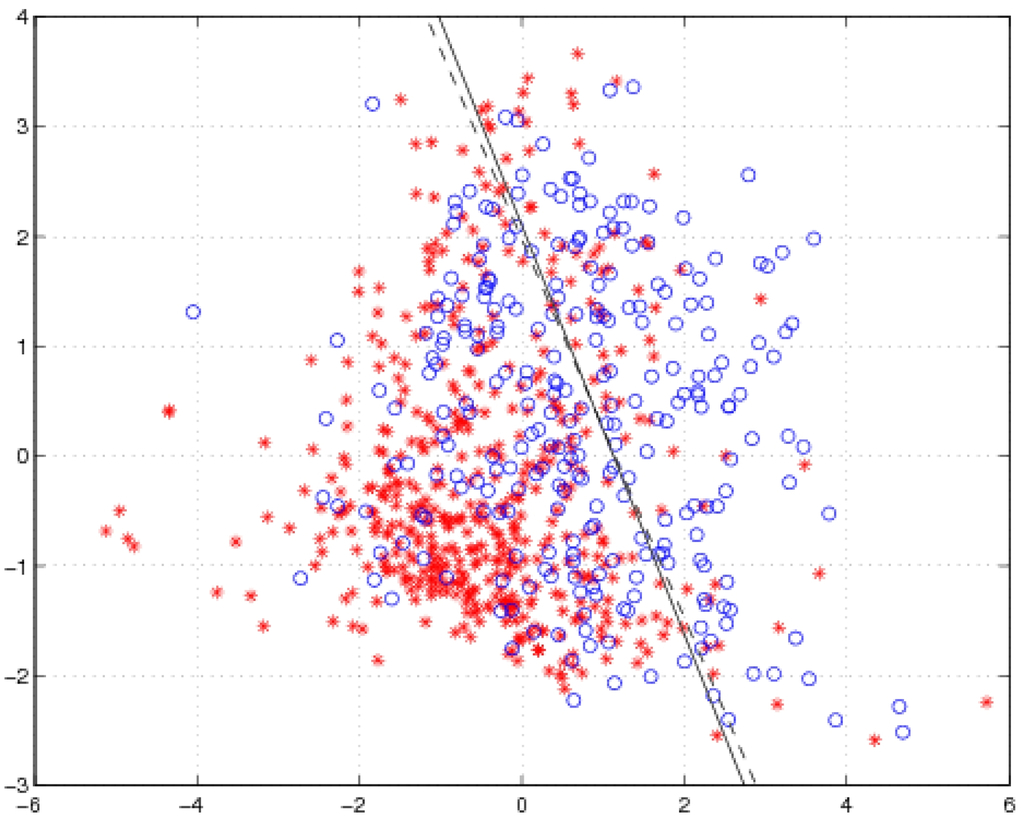
\includegraphics[width=0.6\textwidth]{lec12-26.jpg}
	\end{center}
\end{frame}

% 27
\begin{frame}[c]
	\frametitle{Multiclass Case $(K\geqslant{} 3)$}
	\begin{itemize}
		\item When $K \geqslant{} 3$, $\beta$ is a $(K-1)(p+1)$-vector:
		      \begin{equation*}
			      \beta=
			      \begin{pmatrix}
				      \beta_{10}     \\
				      \beta_{1}      \\
				      \beta_{20}     \\
				      \beta_{2}      \\
				      \vdots         \\
				      \beta_{(K-1)0} \\
				      \beta_{K-1}    \\
			      \end{pmatrix}=
			      \begin{pmatrix}
				      \beta_{10}     \\
				      \beta_{11}     \\
				      \vdots         \\
				      \beta_{1p}     \\
				      \beta_{20}     \\
				      \vdots         \\
				      \beta_{2p}     \\
				      \vdots         \\
				      \beta_{(K-1)0} \\
				      \vdots         \\
				      \beta_{(K-1)p} \\
			      \end{pmatrix}
		      \end{equation*}
	\end{itemize}

\end{frame}

% 28
\begin{frame}[c]
	\frametitle{}
	\begin{itemize}
		\item Let $\bar{\beta}_I=\begin{pmatrix}
				      \beta_{I0} \\
				      \beta_{I}  \\
			      \end{pmatrix}$.
		\item The likelihood function becomes
		      \begin{align*}
			      L(\beta)= & \sum\limits_{i=1}^{N}\log p_{g_i}(x_i;\beta)                                                                           \\
			      =         & \sum\limits_{i=1}^{N} \log \left(\dfrac{e^{\bar{\beta}_{g_i}^Tx_i}}{1+\sum_{I=1}^{K-1}e^{\bar{\beta}_{l}^Tx_i}}\right) \\
			      =         & \sum\limits_{i=1}^{N}
			      \left[\bar{\beta}_{g_i}^Tx_i-
				      \log \left(1+\sum_{I=1}^{K-1}e^{\bar{\beta}_{l}^Tx_i}\right)
				      \right]
		      \end{align*}
	\end{itemize}
\end{frame}

% 29
\begin{frame}[c]
	\frametitle{}
	\begin{itemize}
		\item Note: the indicator function $I(\cdot )$ equals 1 when the argument is true and 0 otherwise.
		\item  First order derivatives:
		      \begin{align*}
			      \dfrac{\partial L(\beta )}{\partial\beta_{kj}}= &
			      \sum\limits_{i=1}^{N}\left[
			      I(g_i=k)x_{ij}-\dfrac{e^{\bar{\beta}_{g_i}^Tx_i}}{1+\sum_{I=1}^{K-1}e^{\bar{\beta}_{l}^Tx_i}}
			      \right]                                                                                                \\
			      =                                               & \sum\limits_{i=1}^{N}x_{ij}(I(g_i=k)-p_k(x_i;\beta))
		      \end{align*}
	\end{itemize}
\end{frame}

% 30
\begin{frame}[c]
	\frametitle{}
	\begin{itemize}
		\item
		      Second order derivatives:
		      \begin{align*}
			        & \dfrac{\partial^2 L(\beta )}{\partial\beta_{kj}\partial\beta_{mn}}                                                                                                      \\
			      = & \sum\limits_{l=1}^{N}x_{ij}\cdot  \dfrac{1}{(1+\sum_{l=1}^{K-1}e^{\bar{\beta}_{I}^Tx_i})^2}\cdot                                                                        \\
			        & \left[-e^{\bar{\beta}_{k}^Tx_i}I(k=m)x_{in}\left(1+\sum\limits_{l=1}^{K-1}e^{\bar{\beta}_{I}^Tx_i}\right)+e^{\bar{\beta}_{k}^Tx_i}e^{\bar{\beta}_{m}^Tx_i}x_{in}\right] \\
			      = & \sum\limits_{i=1}^{N}x_{ij}x_{in}(-p_k(x_i;\beta)I(k=m)+p_k(x_i;\beta)p_m(x_i;\beta))                                                                                   \\
			      = & -\sum\limits_{i=1}^{N}x_{ij}x_{in}p_k(x_i;\beta)[I(k=m)-p_m(x_i;\beta)].
		      \end{align*}
	\end{itemize}
\end{frame}


% 31
\begin{frame}[c]
	\frametitle{}
	\begin{itemize}
		\item  Matrix form.
		      \begin{itemize}
			      \item $\bm{y}$ is the concatenated indicator vector of dimension $N \times (K − 1)$.
			            \begin{gather*}
				            \bm{y}=
				            \begin{pmatrix}
					            \bm{y}_1     \\
					            \bm{y}_2     \\
					            \vdots       \\
					            \bm{y}_{K-1} \\
				            \end{pmatrix}\quad
				            \bm{y}_k=
				            \begin{pmatrix}
					            l(g_1=k) \\
					            l(g_2=k) \\
					            \vdots   \\
					            l(g_N=k) \\
				            \end{pmatrix}
				            \\
				            1\leqslant{}k\leqslant{}K-1
			            \end{gather*}
			      \item  $\bm{p}$ is the concatenated vector of fitted probabilities of dimension $N \times  (K − 1)$.
			            \begin{gather*}
				            \bm{p}=
				            \begin{pmatrix}
					            \bm{p}_1     \\
					            \bm{p}_2     \\
					            \vdots       \\
					            \bm{p}_{K-1} \\
				            \end{pmatrix}\quad
				            \bm{p}_k=
				            \begin{pmatrix}
					            p_k(x_1;\beta) \\
					            p_k(x_2;\beta) \\
					            \vdots         \\
					            p_k(x_N;\beta) \\
				            \end{pmatrix}\\
				            1\leqslant{}k\leqslant{}K-1
			            \end{gather*}
		      \end{itemize}
	\end{itemize}
\end{frame}

% 32
\begin{frame}[c]
	\frametitle{}
	\begin{itemize}
		\item $\tilde{\mathbf{X}}$ is an $N(K − 1) \times (p + 1)(K − 1)$ matrix:
		      \begin{gather*}
			      \tilde{\mathbf{X}}=
			      \begin{pmatrix}
				      \mathbf{X} & \mathbf{0} & \cdots & \mathbf{0} \\
				      \mathbf{0} & \mathbf{X} & \cdots & \mathbf{0} \\
				      \cdots     & \cdots     & \cdots & \cdots     \\
				      \mathbf{0} & \mathbf{0} & \cdots & \mathbf{X} \\
			      \end{pmatrix}
		      \end{gather*}
	\end{itemize}
\end{frame}

% 33
\begin{frame}[c]
	\frametitle{}
	\begin{itemize}
		\item Matrix $\mathbf{W}$ is an $N(K − 1) \times N(K − 1)$ square matrix:
		      \begin{gather*}
			      \mathbf{W}=
			      \begin{pmatrix}
				      \mathbf{W}_{11}      & \mathbf{W}_{12}      & \cdots & \mathbf{W}_{1(K-1)}      \\
				      \mathbf{W}_{21}      & \mathbf{W}_{22}      & \cdots & \mathbf{W}_{2(K-1)}      \\
				      \cdots               & \cdots               & \cdots & \cdots                   \\
				      \mathbf{W}_{(K-1),1} & \mathbf{W}_{(K-1),2} & \cdots & \mathbf{W}_{(K-1),(K-1)} \\
			      \end{pmatrix}
		      \end{gather*}
		\item Each submatrix $\mathbf{W}_{km}$, $1 \leqslant{} k$, $m \leqslant{} K − 1$, is an $N \times N$ diagonal matrix.

		\item  When $k = m$, the $i$ th diagonal element in $\mathbf{W}_{kk}$ is $p_k (x_i;\beta^{old})(1 − p_k (x_i;\beta^{old}))$.

		\item  When $k \neq m$, the $i$ th diagonal element in $\mathbf{W}_{km}$ is $−p_k (x_i;\beta^{old})p_m (x_i;\beta^{old})$.
	\end{itemize}
\end{frame}

% 34
\begin{frame}[c]
	\frametitle{}
	\begin{itemize}
		\item Similarly as with binary classification
		      \begin{gather*}
			      \dfrac{\partial L(\beta )}{\partial\beta}=\tilde{\mathbf{X}}^T(\bm{y}-\bm{p})\\
			      \dfrac{\partial^2 L(\beta )}{\partial\beta\partial\beta^T}=-\tilde{\mathbf{X}}^T\mathbf{W}\tilde{\mathbf{X}}.
		      \end{gather*}
		\item The formula for updating $\beta^{new}$ in the binary classification case holds for multiclass.
		      \begin{gather*}
			      \beta^{new}=(\tilde{\mathbf{X}}^T\mathbf{W}\tilde{\mathbf{X}})^{-1}\tilde{\mathbf{X}}^T\mathbf{W}\bm{z},
		      \end{gather*}
		      where $\bm{z} \xlongequal{\triangle}\tilde{\mathbf{X}}\beta^{old} + \mathbf{W}^{−1}(\bm{y} −\bm{p})$. Or simply:
		      \begin{gather*}
			      \beta^{new}=\beta^{old}+(\tilde{\mathbf{X}}^T\mathbf{W}\tilde{\mathbf{X}})^{-1}\tilde{\mathbf{X}}^T(\bm{y}-\bm{p}).
		      \end{gather*}
	\end{itemize}
\end{frame}

% 35
\begin{frame}[c]
	\frametitle{Computation Issues}
	\begin{itemize}
		\item  Initialization: one option is to use $\beta= 0$.
		\item  Convergence is not guaranteed, but usually is the case.
		\item  Usually, the log-likelihood increases after each iteration, but overshooting can occur.
		\item  In the rare cases that the log-likelihood decreases, cut step size by half.
	\end{itemize}
\end{frame}

% 36
\begin{frame}[c]
	\frametitle{Connection with LDA}
	\begin{itemize}
		\item  Under the model of LDA:
		      \begin{align*}
			        & \log \dfrac{Pr(G=k~|X=x)}{Pr(G=K~|X=x)}                                              \\
			      = & \log \dfrac{\pi_k}{\pi_k}-\dfrac{1}{2}(\mu_k+\mu_K)^T\sum\nolimits^{-1}(\mu_k-\mu_K) \\
			        & +x^T\sum\nolimits^{-1}(\mu_k-\mu_K)                                                  \\
			      = & a_{k0}+a_k^Tx.
		      \end{align*}
		\item  The model of LDA satisfies the assumption of the linear logistic model.
		\item  The linear logistic model only specifies the conditional distribution $Pr(G = k~| X = x)$. No assumption is made about $Pr(X)$.
	\end{itemize}
\end{frame}

% 37
\begin{frame}[c]
	\frametitle{}
	\begin{itemize}
		\item  The LDA model specifies the joint distribution of $X$ and $G$. $Pr(X)$ is a mixture of Gaussians:
		      \begin{eqnarray*}
			      Pr(x)=\sum\limits_{k=1}^{K}\pi_k\phi\left(X;\mu_k,\sum\right).
		      \end{eqnarray*}
		      where $\phi$ is the Gaussian density function.
		\item  Linear logistic regression maximizes the conditional likelihood of $G$ given $X$: $Pr(G = k~| X = x)$.
		\item  LDA maximizes the joint likelihood of $G$ and $X$: $Pr(X = x,G = k)$.
	\end{itemize}
\end{frame}

% 38
\begin{frame}[c]
	\frametitle{}
	\begin{itemize}
		\item  If the additional assumption made by LDA is appropriate, LDA tends to estimate the parameters more efficiently by using more information about the data.

		\item  Samples without class labels can be used under the model of LDA.

		\item  LDA is not robust to gross outliers.

		\item  As logistic regression relies on fewer assumptions, it seems to be more robust.

		\item  In practice, logistic regression and LDA often give similar results.
	\end{itemize}
\end{frame}

% 39
\begin{frame}[c]
	\frametitle{Simulation}
	\begin{itemize}
		\item Assume input $X$ is 1-D.
		\item  Two classes have equal priors and the class-conditional densities of $X$ are shifted versions of each other.

		\item  Each conditional density is a mixture of two normals:
		      \begin{itemize}
			      \item
			            Class 1 (red): $0.6N\left(−2,\frac14\right)+0.4N(0,1)$.
			      \item
			            Class 2 (blue): $0.6N\left(0,\frac14\right)+0.4N(2,1)$.
		      \end{itemize}
		\item The class-conditional densities are shown below.
	\end{itemize}
\end{frame}

% 40
\begin{frame}[c]
	\frametitle{}
	\begin{center}
		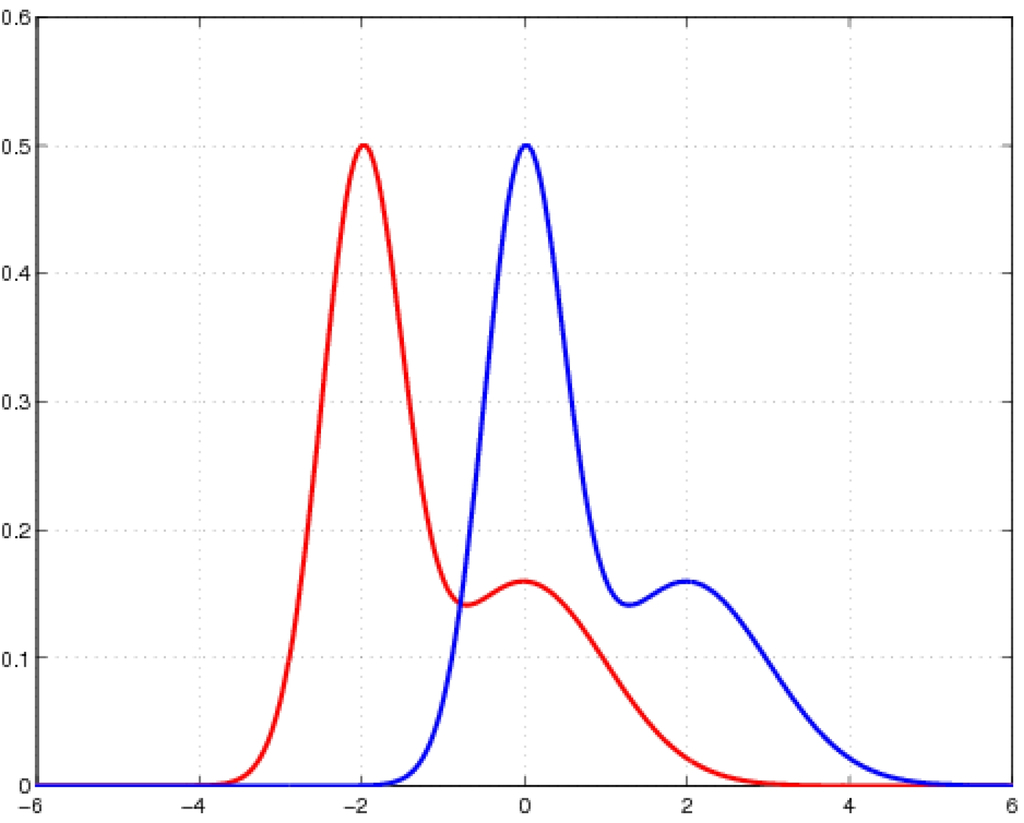
\includegraphics[width=0.7\textwidth]{lec12-40.jpg}
	\end{center}
\end{frame}

% 41
\begin{frame}[c]
	\frametitle{LDA Result}
	\begin{itemize}
		\item Training data set: 2000 samples for each class.

		\item  Test data set: 1000 samples for each class.

		\item The estimation by LDA: $\hat{\mu}_1 = −1.1948$, $\hat{\mu}_2 = 0.8224$, $\hat{\sigma}_2 = 1.5268$. Boundary value between the two classes is $(\hat{\mu}_1 +\hat{\mu}_ 2)/2 =−0.1862$.

		\item  The classification error rate on the test data is 0.2315.
		\item
		      Based on the true distribution, the Bayes (optimal) boundary value between the two classes is $−0.7750$ and the error rate is 0.1765.
	\end{itemize}
\end{frame}

% 42
\begin{frame}[c]
	\frametitle{}
	\begin{center}
		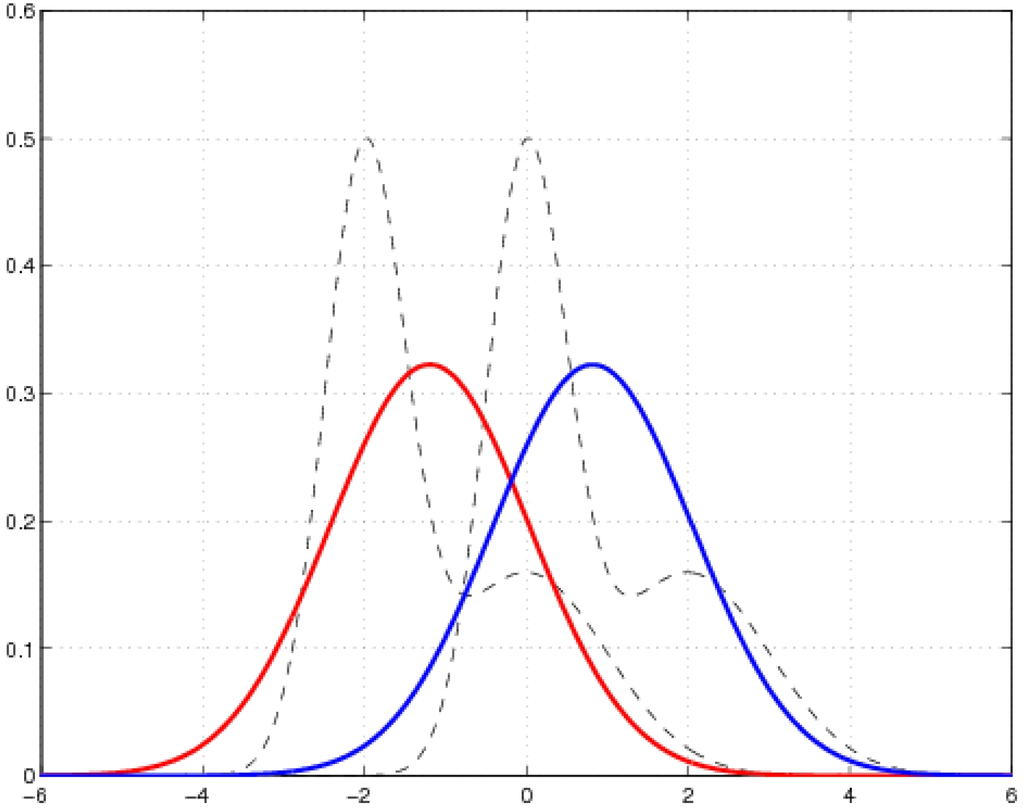
\includegraphics[width=0.7\textwidth]{lec12-42.jpg}
	\end{center}
\end{frame}

% 43
\begin{frame}[c]
	\frametitle{Logistic Regression Result}
	\begin{itemize}
		\item  Linear logistic regression obtains
		      \begin{gather*}
			      \beta=(-0.3288,-1.3275)^T.
		      \end{gather*}
		      The boundary value satisfies $−0.3288 − 1.3275X = 0$, hence equals $−0.2477$.

		\item The error rate on the test data set is 0.2205.

		\item  The estimated posterior probability is:
		      \begin{gather*}
			      Pr(G=1~|X=x)=\dfrac{e^{-0.3288-13275x}}{1+e^{-0.3288-1.3275x}}.
		      \end{gather*}
	\end{itemize}

\end{frame}

% 44
\begin{frame}[c]
	\frametitle{}
	The estimated posterior probability $Pr(G = 1~| X = x)$ and its true value based on the true distribution are compared in the graph below.
	\begin{center}
		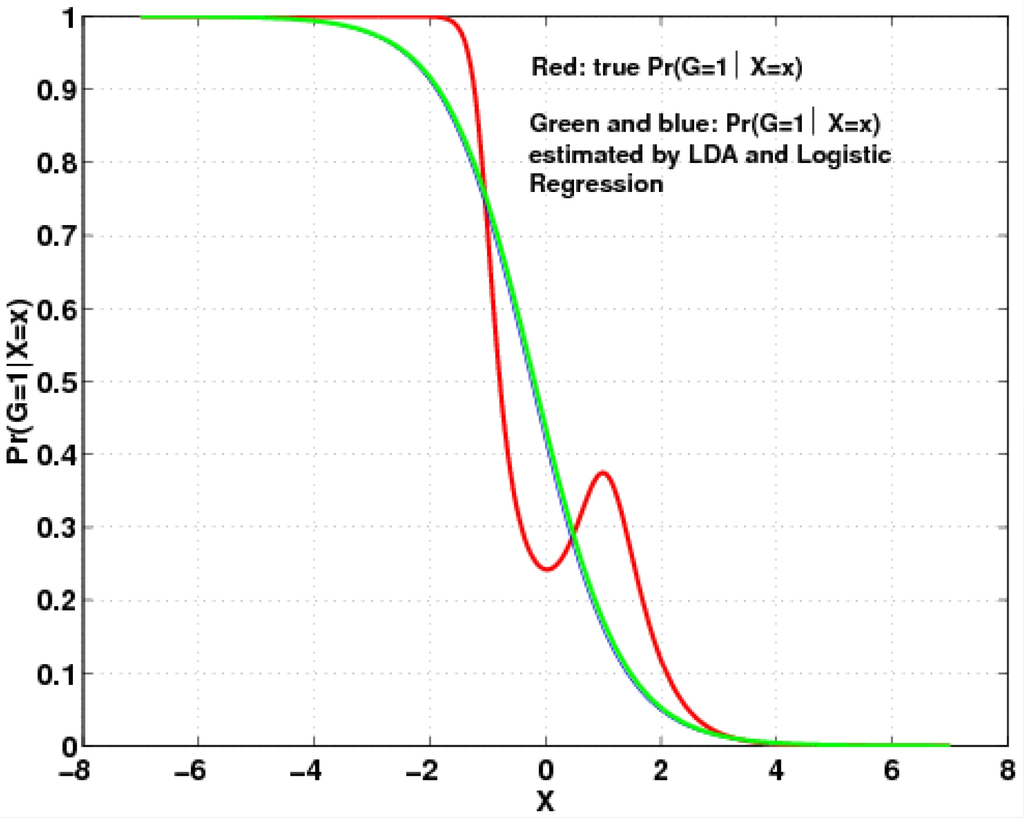
\includegraphics[width=0.6\textwidth]{lec12-44.jpg}
	\end{center}
\end{frame}
\begin{frame}
	\begin{center}
		\chuhao Thank you! %\fontspec{LHANDW.TTF}
	\end{center}
\end{frame}
\end{document}
